% -----------------------------*- LaTeX -*------------------------------
\documentclass[UTF8]{report}
% ------------------------------------------------------------------------
% Packages
% ------------------------------------------------------------------------
\usepackage{ctex} % 支持中文
\usepackage[body={7in, 9in},left=1in,right=1in]{geometry} % 改变页边距
\usepackage{amsmath} % AMS 的数学宏包
\usepackage{amsfonts} % AMS 的数学字体宏包
\usepackage{amssymb} % AMS 符号库
\usepackage{bm} % 数学公式中的黑斜体
\usepackage{amsthm} % AMS 的定理环境宏包
\usepackage{graphicx} % 插图
\usepackage{subfigure} % 插子图
\usepackage{nicefrac} % 好看的分数
\usepackage{mathrsfs} % mathscr font
\usepackage{caption} % caption
\usepackage{algorithm,algorithmicx} % 伪代码支持宏包
\usepackage[noend]{algpseudocode} % 伪代码
\usepackage{fancyhdr} % 设置页眉、页脚
\usepackage{adjustbox} % 图片尺寸自动调整
\usepackage{esint} % 积分符号
\usepackage{mathtools} % 数学宏包的重要补充
\usepackage{upgreek} % 数学环境的直立希腊字母
\usepackage{enumitem} % 使用enumitem宏包, 改变列表项的格式
\usepackage{color} % 支持彩色
\usepackage{extarrows} % 任意长度的箭头
\usepackage{tikz} % 绘图
\usepackage{forest} % 绘树
\usepackage{xcolor} % 颜色宏包
\usepackage{breqn} % 公式自动换行
\usepackage{fontsize} % 字体大小
\usepackage[framemethod=TikZ]{mdframed} % 给文字加框
\usepackage{fontspec} % 字体库
\usepackage{bigstrut} % 用于表格中的换行
\usepackage{multirow} % 表格中多行单元格合并
\usepackage{multicol} % 表格中多列单元格合并
\usepackage{longtable} % 长表格
\usepackage{rotating} % 旋转图形和表格      以上三者用于绘制三线表
\usepackage{booktabs} % 三线表宏包
\usepackage{scribe} % Scribe 模板
\usepackage{diagbox} % 表格斜线
\usepackage{listings} % 插入代码
\usepackage{verbatim} % 多行注释
\usepackage{ifplatform} % 检测编译平台
\usepackage{pifont} % 圆圈数字
\usetikzlibrary{shapes.geometric, arrows} % 引入流程图需要的库
\usetikzlibrary{automata} % 引入automata库
\usetikzlibrary{shapes,arrows,positioning,chains} % 引入positioning库
% ------------------------------------------------------------------------
% Macros
% ------------------------------------------------------------------------
%~~~~~~~~~~~~~~~
% Utility latin
%~~~~~~~~~~~~~~~
\newcommand{\ie}{\textit{i.e.}}
\newcommand{\eg}{\textit{e.g.}}
%~~~~~~~~~~~~~~~
% Environment shortcuts
%~~~~~~~~~~~~~~~
\newcommand{\balign}[1]{\ealign{\begin{align}#1\end{align}}}
\newcommand{\baligns}[1]{\ealigns{\begin{align*}#1\end{align*}}}
\newcommand{\bitemize}[1]{\eitemize{\begin{itemize}#1\end{itemize}}}
\newcommand{\benumerate}[1]{\eenumerate{\begin{enumerate}#1\end{enumerate}}}
%~~~~~~~~~~~~~~~
% Text with quads around it
%~~~~~~~~~~~~~~~
\newcommand{\qtext}[1]{\quad\text{#1}\quad}
%~~~~~~~~~~~~~~~
% Shorthand for math formatting
%~~~~~~~~~~~~~~~
\newcommand{\mbb}[1]{\mathbb{#1}}
\newcommand{\mbi}[1]{\boldsymbol{#1}} % Bold and italic (math bold italic)
\newcommand{\mbf}[1]{\mathbf{#1}}
\newcommand{\mc}[1]{\mathcal{#1}}
\newcommand{\mrm}[1]{\mathrm{#1}}
\newcommand{\tbf}[1]{\textbf{#1}}
\newcommand{\tsc}[1]{\textsc{#1}}
%\def\\langle {{\langle }}
%\def\\rangle {{\rangle }}
\newcommand{\sT}{\sf T}
\newcommand{\grad}{\nabla}
\newcommand{\Proj}{\Pi}
%~~~~~~~~~~~~~~~
% Common sets 定义数集符号
%~~~~~~~~~~~~~~~
\newcommand{\R}{\mathbb{R}}
\newcommand{\Z}{\mathbb{Z}}
\newcommand{\Q}{\mathbb{Q}}
\newcommand{\N}{\mathbb{N}}
\newcommand{\C}{\mathbb{C}}
\newcommand{\reals}{\mathbb{R}} % Real number symbol
\newcommand{\integers}{\mathbb{Z}} % Integer symbol
\newcommand{\rationals}{\mathbb{Q}} % Rational numbers
\newcommand{\naturals}{\mathbb{N}} % Natural numbers
\newcommand{\complex}{\mathbb{C}} % Complex numbers
%~~~~~~~~~~~~~~~
% Common functions
%~~~~~~~~~~~~~~~
\renewcommand{\exp}[1]{\operatorname{exp}\left(#1\right)} % Exponential
\newcommand{\indic}[1]{\mbb{I}\left(#1\right)} % Indicator function
\newcommand{\indicsub}[2]{\mbb{I}_{#2}\left(#1\right)} % Indicator function
\newcommand{\argmax}{\mathop\mathrm{arg\, max}} % Defining math symbols
\newcommand{\argmin}{\mathop\mathrm{arg\, min}}
\renewcommand{\arccos}{\mathop\mathrm{arccos}}
\newcommand{\dom}{\mathop\mathrm{dom}} % Domain
\newcommand{\range}{\mathop\mathrm{range}} % Range
\newcommand{\diag}{\mathop\mathrm{diag}}
\newcommand{\tr}{\mathop\mathrm{tr}}
\newcommand{\abs}{\mathop\mathrm{abs}}
\newcommand{\card}{\mathop\mathrm{card}}
\newcommand{\sign}{\mathop\mathrm{sign}}
\newcommand{\prox}{\mathrm{prox}} % prox
\newcommand{\rank}[1]{\mathrm{rank}(#1)}
\newcommand{\supp}[1]{\mathrm{supp}(#1)}
\newcommand{\norm}[1]{\lVert#1\rVert}
%~~~~~~~~~~~~~~~
% Common probability symbols
%~~~~~~~~~~~~~~~
\newcommand{\family}{\mathcal{P}} % probability family / statistical model
\newcommand{\iid}{\stackrel{\mathrm{iid}}{\sim}}
\newcommand{\ind}{\stackrel{\mathrm{ind}}{\sim}}
\newcommand{\E}{\mathbb{E}} % Expectation symbol
\newcommand{\Earg}[1]{\E\left[#1\right]}
\newcommand{\Esubarg}[2]{\E_{#1}\left[#2\right]}
\renewcommand{\P}{\mathbb{P}} % Probability symbol
\newcommand{\Parg}[1]{\P\left(#1\right)}
\newcommand{\Psubarg}[2]{\P_{#1}\left[#2\right]}
%\newcommand{\Cov}{\mrm{Cov}} % Covariance symbol
%\newcommand{\Covarg}[1]{\Cov\left[#1\right]}
%\newcommand{\Covsubarg}[2]{\Cov_{#1}\left[#2\right]}
%\newcommand{\model}{\mathcal{P}} % probability family / statistical model
%~~~~~~~~~~~~~~~
% Distributions
%~~~~~~~~~~~~~~~
%\newcommand{\Gsn}{\mathcal{N}}
%\newcommand{\Ber}{\textnormal{Ber}}
%\newcommand{\Bin}{\textnormal{Bin}}
%\newcommand{\Unif}{\textnormal{Unif}}
%\newcommand{\Mult}{\textnormal{Mult}}
%\newcommand{\NegMult}{\textnormal{NegMult}}
%\newcommand{\Dir}{\textnormal{Dir}}
%\newcommand{\Bet}{\textnormal{Beta}}
%\newcommand{\Gam}{\textnormal{Gamma}}
%\newcommand{\Poi}{\textnormal{Poi}}
%\newcommand{\HypGeo}{\textnormal{HypGeo}}
%\newcommand{\GEM}{\textnormal{GEM}}
%\newcommand{\BP}{\textnormal{BP}}
%\newcommand{\DP}{\textnormal{DP}}
%\newcommand{\BeP}{\textnormal{BeP}}
%\newcommand{\Exp}{\textnormal{Exp}}
%~~~~~~~~~~~~~~~
% Theorem-like environments
%~~~~~~~~~~~~~~~
%\theoremstyle{definition}
%\newtheorem{definition}{Definition}
%\newtheorem{example}{Example}
%\newtheorem{problem}{Problem}
%\newtheorem{lemma}{Lemma}
%~~~~~~~~~~~~~~~
% 组合数学的模板和作业里用到的一些宏包和自定义命令
%~~~~~~~~~~~~~~~
\renewcommand{\emph}[1]{\begin{kaishu}#1\end{kaishu}}
\newcommand{\falfac}[1]{^{\underline{#1}}}
\newcommand{\binomfrac}[2]{\frac{#1^{\underline{#2}}}{#2!}}
\newcommand{\ceil}[1]{\left\lceil #1 \right\rceil}
\newcommand{\floor}[1]{\left\lfloor #1 \right\rfloor}
\newcommand{\suminfty}[2]{\sum_{#1=#2}^{\infty}}
\newcommand{\suminftyk}[0]{\sum_{k=0}^{\infty}}
\newcommand{\sumint}[3]{\sum_{#1=#2}^{#3}}
\newcommand{\sumintk}[2]{\sum_{k=#1}^{#2}}
\newcommand{\suminti}[2]{\sum_{i=#1}^{#2}}
%~~~~~~~~~~~~~~~
% 定义新命令
%~~~~~~~~~~~~~~~
\newcommand*{\unit}[1]{\mathop{}\!\mathrm{#1}}
\newcommand*{\dif}{\mathop{}\!\mathrm{d}}%微分算子 d
\newcommand*{\pdif}{\mathop{}\!\partial}%偏微分算子
\newcommand*{\cdif}{\mathop{}\!\nabla}%协变导数、nabla 算子
\newcommand*{\laplace}{\mathop{}\!\Delta}%laplace 算子
\newcommand*{\deri}[1]{\mathrm{d} #1}
\newcommand*{\deriv}[2]{\frac{\mathrm{d} #1}{\mathrm{d} {#2}}}
\newcommand*{\derivh}[3]{\frac{\mathrm{d}^{#1} #2}{\mathrm{d} {#3^{#1}}}}
\newcommand*{\pderiv}[2]{\frac{\partial #1}{\partial {#2}}}
\newcommand*{\pderivh}[3]{\frac{\partial^{#1} #2}{\partial {#3^{#1}}}}
\newcommand*{\dderiv}[2]{\dfrac{\mathrm{d} #1}{\mathrm{d} {#2}}}
\newcommand*{\dderivh}[3]{\dfrac{\mathrm{d}^{#1} #2}{\mathrm{d} {#3^{#1}}}}
\newcommand*{\dpderiv}[2]{\dfrac{\partial #1}{\partial {#2}}}
\newcommand*{\dpderivh}[3]{\dfrac{\partial^{#1} #2}{\partial {#3^{#1}}}}
\newcommand{\me}[1]{\mathrm{e}^{#1}}%e 指数
\newcommand{\mi}{\mathrm{i}}%虚数单位
%\newcommand{\mc}{\mathrm{c}}%光速 定义与mathcal冲突
\newcommand{\red}[1]{\textcolor{red}{#1}}
\newcommand{\blue}[1]{\textcolor{blue}{#1}}
%\newcommand{\Rome}[1]{\setcounter{rome}{#1}\Roman{rome}}
%~~~~~~~~~~~~~~~
% 公式环境中箭头符号的简写
%~~~~~~~~~~~~~~~
\newcommand{\ra}{\rightarrow}
\newcommand{\Ra}{\Rightarrow}
\newcommand{\la}{\leftarrow}
\newcommand{\La}{\Leftarrow}
\newcommand{\lra}{\leftrightarrow}
\newcommand{\Lra}{\Leftrightarrow}
\newcommand{\lgla}{\longleftarrow}
\newcommand{\Lgla}{\Longleftarrow}
\newcommand{\lgra}{\longrightarrow}
\newcommand{\Lgra}{\Longrightarrow}
\newcommand{\lglra}{\longleftrightarrow}
\newcommand{\Lglra}{\Longleftrightarrow}
%~~~~~~~~~~~~~~~
% 一些数学的环境设置
%~~~~~~~~~~~~~~~
%\newcounter{counter_exm}\setcounter{counter_exm}{1}
%\newcounter{counter_prb}\setcounter{counter_prb}{1}
%\newcounter{counter_thm}\setcounter{counter_thm}{1}
%\newcounter{counter_lma}\setcounter{counter_lma}{1}
%\newcounter{counter_dft}\setcounter{counter_dft}{1}
%\newcounter{counter_clm}\setcounter{counter_clm}{1}
%\newcounter{counter_cly}\setcounter{counter_cly}{1}
\newtheorem{theorem}{{\hskip 1.7em \bf 定理}}
\newtheorem{lemma}[theorem]{\hskip 1.7em 引理}
\newtheorem{proposition}[theorem]{\hskip 1.7em 命题}
\newtheorem{claim}[theorem]{\hskip 1.7em 断言}
\newtheorem{corollary}[theorem]{\hskip 1.7em 推论}
% \newcommand{\problem}[1]{{\setlength{\parskip}{10pt}\noindent \bf{#1}}}
\newenvironment{solution}{{\noindent \bf 解 \quad}}{}
\newenvironment{remark}{{\noindent \bf 注 \quad}}{}
\newenvironment{definition}{{\noindent \bf 定义 \quad}}{}
\renewenvironment{proof}{{\setlength{\parskip}{7pt}\noindent\hskip 2em \bf 证明 \quad}}{\hfill$\qed$\par}
\newenvironment{example}{{\noindent\bf 例 \quad}}{\hfill$\qed$\par}
%\newenvironment{concept}[1]{{\bf #1\quad} \begin{kaishu}} {\end{kaishu}\par}
%~~~~~~~~~~~~~~~
% 本.tex文档中特殊定义命令
%~~~~~~~~~~~~~~~
\newcommand{\lno}[1]{\overline{#1}}
\newcommand{\NP}{\mathrm{NP}}
\newcommand{\coNP}{\mathrm{coNP}}
% \newcommand{\ISO}{\mathrm{ISO}}
\newcommand{\SAT}{\mathrm{SAT}}
\newcommand{\USAT}{\mathrm{USAT}}
% \newcommand{\threeSAT}{\mathrm{3\text{-}SAT}}
\renewcommand{\P}{\mathrm{P}}
% \mathchardef\mhyphen="2D
% \newcommand{\CNF}{\mathrm{CNF}}
% \newcommand{\DNF}{\mathrm{DNF}}
% \newcommand{\SetSp}{\mathrm{SET\text{-}SPLITTING}}
% \newcommand{\PUZZLE}{\mathrm{PUZZLE}}
% \newcommand{\SPATH}{\mathrm{SPATH}}
% \newcommand{\LPATH}{\mathrm{LPATH}}
% \newcommand{\UHAMPATH}{\mathrm{UHAMPATH}}
\newcommand{\SPACE}{\mathrm{SPACE}}
\newcommand{\NSPACE}{\mathrm{NSPACE}}
\newcommand{\PSPACE}{\mathrm{PSPACE}}
\newcommand{\NPSPACE}{\mathrm{NPSPACE}}
\newcommand{\DFA}{\mathrm{DFA}}
\newcommand{\NFA}{\mathrm{NFA}}
\newcommand{\TQBF}{\mathrm{TQBF}}
% \newcommand{\L}{\mathrm{L}}
\renewcommand{\O}{\mathrm{O}}
\newcommand{\NL}{\mathrm{NL}}
\newcommand{\coNL}{\mathrm{coNL}}
\newcommand{\LADDER}{\mathrm{LADDER_{DFA}}}
\newcommand{\hd}{\mathrm{\text{-}hard}}
\newcommand{\ADD}{\mathrm{ADD}}
\newcommand{\STCN}{\mathrm{STRONGLY\text{-}CONNECTED}}
\newcommand{\PATH}{\mathrm{PATH}}
\newcommand{\A}{\mathrm{A}}
%使用align环境公式换页
\allowdisplaybreaks[4]

\definecolor{dkgreen}{rgb}{0,0.6,0}
\definecolor{gray}{rgb}{0.5,0.5,0.5}
\definecolor{mauve}{rgb}{0.58,0,0.82}
\lstset{
  frame=tb,
  aboveskip=3mm,
  belowskip=3mm,
  showstringspaces=false,
  columns=flexible,
  framerule=1pt,
  rulecolor=\color{gray!35},
  backgroundcolor=\color{gray!5},
  basicstyle={\small\ttfamily},
  numbers=none,
  numberstyle=\tiny\color{gray},
  keywordstyle=\color{blue},
  commentstyle=\color{dkgreen},
  stringstyle=\color{mauve},
  breaklines=true,
  breakatwhitespace=true,
  tabsize=3,
}

\tikzstyle{startstop} = [rectangle, rounded corners, minimum width=3cm, minimum height=1cm,text centered, draw=black, fill=red!30]
\tikzstyle{process} = [rectangle, minimum width=3cm, minimum height=1cm, text centered, draw=black, fill=orange!30]
\tikzstyle{decision} = [diamond, minimum width=3cm, minimum height=1cm, text centered, draw=black, fill=green!30]
\tikzstyle{arrow} = [thick,->,>=stealth]

\ifwindows
    \setmainfont{Times New Roman}
    \setsansfont{Times New Roman}
    \setmonofont{Consolas}
    \setCJKmainfont{SimHei}
    \setCJKsansfont{SimSun}
    \setCJKmonofont{FangSong}
\fi

\ifmacosx
    \setmainfont{Times New Roman}
    \setsansfont{Times New Roman}
    \setmonofont{Menlo}
    \setCJKmainfont{STHeiti}
    \setCJKsansfont{STSong}
    \setCJKmonofont{STFangsong}
\fi

\punctstyle{kaiming}

\begin{document}

\pagestyle{fancy}

\reporttype{Report}                 % required
\course{Lab of Computer Network} 				% optional
\coursetitle{MOSPF}	    % optional
\semester{Fall 2024}			    % optional
\lecturer{Wu Qinghua}			% optional
\scribe{2022K8009929010 Zhang Jiawei}			% required
\lecturenumber{9}				% required (must be a number)
\lecturedate{Novmeber 7}			% required (omit year)
\maketitle

\section{实验内容}

\begin{enumerate}
    \item 实验内容一
    \begin{itemize}
        \item 基于已有代码框架,实现路由器生成和处理mOSPF Hello/LSU消息的相关操作,构建一致性链路状态数据库;
        \item 运行实验
        \begin{itemize}
            \item 运行网络拓扑(topo.py)
            \item 在各个路由器节点上执行disable_arp.sh, disable_icmp.sh, disable_ip_forward.sh,禁止协议栈的相应功能
            \item 运行./mospfd,使得各个节点生成一致的链路状态数据库。
        \end{itemize}
    \end{itemize}
    \item 实验内容二
    \begin{itemize}
        \item 基于实验一,实现路由器计算路由表项的相关操作;
        \item 运行实验
        \begin{itemize}
            \item 运行网络拓扑(topo.py)
            \item 在各个路由器节点上执行disable_arp.sh, disable_icmp.sh, disable_ip_forward.sh,禁止协议栈的相应功能
            \item 运行./mospfd,使得各个节点生成一致的链路状态数据库
            \item 等待一段时间后,每个节点生成完整的路由表项
            \item 在节点h1上ping/traceroute节点h2
            \item 关掉某节点或链路,等一段时间后,再次用h1去traceroute节点h2。
        \end{itemize}
    \end{itemize}
\end{enumerate}

\section{实验过程}

\subsection{链路邻居发现}

对于每一个链路上的路由器节点,都会从各个端口以5秒为周期发送Hello消息,以便发现邻居节点。Hello消息包括了发送节点的ID、端口的子网掩码等等信息。需要注意一点,Hello消息的目的IP地址是224.0.0.5,目的MAC地址是01:00:5e:00:00:05,这是因为Hello消息是多播消息,需要发送给多播组。再接上各层头部,即可发送。具体代码如下:

\begin{lstlisting}[language=C]
    void *sending_mospf_hello_thread(void *param)
    {
        // fprintf(stdout, "TODO: send mOSPF Hello message periodically.\n");
        while (1)
        {
            sleep(MOSPF_DEFAULT_HELLOINT);
            pthread_mutex_lock(&mospf_lock);
    
            iface_info_t *iface = NULL;
            list_for_each_entry(iface, &instance->iface_list, list) {
                int mospf_len = MOSPF_HDR_SIZE + MOSPF_HELLO_SIZE;
                int packet_len = ETHER_HDR_SIZE + IP_BASE_HDR_SIZE + mospf_len;
                char *packet = (char *)malloc(packet_len);
                struct ether_header *ethdr = (struct ether_header *)packet;
                struct iphdr *iphdr = packet_to_ip_hdr(packet);
                struct mospf_hdr *mospfhdr = (struct mospf_hdr *)((char *)iphdr + IP_BASE_HDR_SIZE);
                struct mospf_hello *hello = (struct mospf_hello *)((char *)mospfhdr + MOSPF_HDR_SIZE);
    
                memset(packet, 0, packet_len);
    
                mospf_init_hello(hello, iface->mask);
                mospf_init_hdr(mospfhdr, MOSPF_TYPE_HELLO, mospf_len, instance->router_id, instance->area_id);
                mospfhdr->checksum = mospf_checksum(mospfhdr);
    
                ip_init_hdr(iphdr, iface->ip, MOSPF_ALLSPFRouters, packet_len - ETHER_HDR_SIZE, IPPROTO_MOSPF);
    
                memcpy(ethdr->ether_dhost, "\x01\x00\x5e\x00\x00\x05", ETH_ALEN);
                memcpy(ethdr->ether_shost, iface->mac, ETH_ALEN);
                ethdr->ether_type = htons(ETH_P_IP);
    
                iface_send_packet(iface, packet, packet_len);
            }
    
            pthread_mutex_unlock(&mospf_lock);
        }
        
        return NULL;
    }
\end{lstlisting}

当某个路由器节点接收到邻居节点发来的Hello消息时,会根据Hello消息中的信息更新邻居节点的信息。若源节点在自身邻居列表中,则更新对应存活时间等等数据项;若源节点不在自身邻居列表中,则将其加入邻居列表,导致邻居列表变动,所以还需要发送LSU消息通知其他节点。具体代码如下:

\begin{lstlisting}[language=C]
    void handle_mospf_hello(iface_info_t *iface, const char *packet, int len)
    {
        // fprintf(stdout, "TODO: handle mOSPF Hello message.\n");
        struct iphdr *iphdr = (struct iphdr *)(packet + ETHER_HDR_SIZE);
        struct mospf_hdr *mospfhdr = (struct mospf_hdr *)((char *)iphdr + IP_HDR_SIZE(iphdr));
        struct mospf_hello *hello = (struct mospf_hello *)((char *)mospfhdr + MOSPF_HDR_SIZE);
        pthread_mutex_lock(&mospf_lock);
    
        mospf_nbr_t *nbr = NULL;
        list_for_each_entry(nbr, &iface->nbr_list, list) {
            if (nbr->nbr_id == ntohl(mospfhdr->rid)) {
                nbr->alive = 0;
                nbr->nbr_ip = ntohl(iphdr->saddr);
                nbr->nbr_mask = ntohl(hello->mask);
    
                pthread_mutex_unlock(&mospf_lock);
                return;
            }
        }
    
        nbr = (mospf_nbr_t *)malloc(sizeof(mospf_nbr_t));
        nbr->nbr_id = ntohl(mospfhdr->rid);
        nbr->nbr_ip = ntohl(iphdr->saddr);
        nbr->nbr_mask = ntohl(hello->mask);
        nbr->alive = 0;
        init_list_head(&nbr->list);
        list_add_tail(&nbr->list, &iface->nbr_list);
        iface->num_nbr++;
    
        send_mospf_lsu_packet();
        pthread_mutex_unlock(&mospf_lock);
    }
\end{lstlisting}

此外,邻居列表还需要一个老化操作,如果列表中的节点在3*hello-interval时间内未更新,则将其删除,也导致邻居列表变动,需要发送LSU消息通知其他节点。具体代码如下:

\begin{lstlisting}[language=C]
    void *checking_nbr_thread(void *param)
    {
        // fprintf(stdout, "TODO: neighbor list timeout operation.\n");
        while (1)
        {
            sleep(1);
            pthread_mutex_lock(&mospf_lock);
    
            int delete = 0;
            iface_info_t *iface = NULL;
            list_for_each_entry(iface, &instance->iface_list, list) {
                mospf_nbr_t *nbr = NULL;
                mospf_nbr_t *nbr_q = NULL;
                list_for_each_entry_safe(nbr, nbr_q, &iface->nbr_list, list) {
                    if (nbr->alive > 3 * iface->helloint){
                        delete = 1;
                        iface->num_nbr--;
                        list_delete_entry(&nbr->list);
                        free(nbr);
                    }
                    else
                        nbr->alive++;
                }
            }
    
            if (delete)
                send_mospf_lsu_packet();
            
            pthread_mutex_unlock(&mospf_lock);
        }
        
        return NULL;
    }
\end{lstlisting}

\subsection{链路状态洪泛}

路由器节点每隔一段时间就会发送一次LSU消息,以便通知其他节点自身的链路状态。我将发送过程封装成一个函数,发送完成后打印节点数据库信息。具体代码如下:

\begin{lstlisting}[language=C]
    void *sending_mospf_lsu_thread(void *param)
    {
        // fprintf(stdout, "TODO: send mOSPF LSU message periodically.\n");
        while (1)
        {
            sleep(MOSPF_DEFAULT_LSUINT);
            pthread_mutex_lock(&mospf_lock);
            send_mospf_lsu_packet();
            print_database();
            pthread_mutex_unlock(&mospf_lock);
        }
        return NULL;
    }    
\end{lstlisting}

发送函数的具体实现如下,首先生成要发送的LSA部分,LSA消息的个数为所有邻居节点个数加上无邻居节点的接口个数,内容包括网络地址、子网掩码、邻居节点ID(无邻居则为0)。然后生成LSU消息,对于各个端口,复制其相应的LSA消息,添加头部信息,向邻居节点发送。具体代码如下:

\begin{lstlisting}[language=C]
    void send_mospf_lsu_packet()
    {
        int lsa_num = 0;
        iface_info_t *iface = NULL;
        list_for_each_entry(iface, &instance->iface_list, list) {
            lsa_num += iface->num_nbr ? iface->num_nbr : 1;
        }
    
        int mospf_len = MOSPF_HDR_SIZE + MOSPF_LSU_SIZE + lsa_num * MOSPF_LSA_SIZE;
        char *packet = (char *)malloc(mospf_len);
        memset(packet, 0, mospf_len);
        struct mospf_hdr *mospfhdr = (struct mospf_hdr *)packet;
        struct mospf_lsu *lsu = (struct mospf_lsu *)((char *)mospfhdr + MOSPF_HDR_SIZE);
        struct mospf_lsa *lsa = (struct mospf_lsa *)((char *)lsu + MOSPF_LSU_SIZE);
    
        iface = NULL;
        list_for_each_entry(iface, &instance->iface_list, list) {
            if (iface->num_nbr) {
                mospf_nbr_t *nbr = NULL;
                list_for_each_entry(nbr, &iface->nbr_list, list) {
                    lsa->network = iface->ip & iface->mask;
                    lsa->mask = iface->mask;
                    lsa->rid = nbr->nbr_id;
                    lsa++;
                }
            }
            else {
                lsa->network = iface->ip & iface->mask;
                lsa->mask = iface->mask;
                lsa->rid = 0;
                lsa++;
            }
        }
    
        mospf_init_lsu(lsu, lsa_num);
        instance->sequence_num++;
    
        mospf_init_hdr(mospfhdr, MOSPF_TYPE_LSU, mospf_len, instance->router_id, instance->area_id);
        mospfhdr->checksum = mospf_checksum(mospfhdr);
    
        iface = NULL;
        list_for_each_entry(iface, &instance->iface_list, list) {
            if (iface->num_nbr) {
                mospf_nbr_t *nbr = NULL;
                list_for_each_entry(nbr, &iface->nbr_list, list) {
                    char *packet_send = (char *)malloc(ETHER_HDR_SIZE + IP_BASE_HDR_SIZE + mospf_len);
                    struct ether_header *ethdr = (struct ether_header *)packet_send;
                    struct iphdr *iphdr = (struct iphdr *)(packet_send + ETHER_HDR_SIZE);
                    char *mospf_message = packet_send + ETHER_HDR_SIZE + IP_BASE_HDR_SIZE;
    
                    memset(packet_send, 0, ETHER_HDR_SIZE + IP_BASE_HDR_SIZE + mospf_len);
                    memcpy(mospf_message, packet, mospf_len);
                    ip_init_hdr(iphdr, iface->ip, nbr->nbr_ip, mospf_len + IP_BASE_HDR_SIZE, IPPROTO_MOSPF);
                    memcpy(ethdr->ether_shost, iface->mac, ETH_ALEN);
                    ethdr->ether_type = htons(ETH_P_IP);
    
                    iface_send_packet_by_arp(iface, nbr->nbr_ip, packet_send, ETHER_HDR_SIZE + IP_BASE_HDR_SIZE + mospf_len);
                }
            }
        }
        free(packet);
    }    
\end{lstlisting}

当某个路由器节点接收到LSU消息时,先检查是否是自身发送的,若是则丢弃。若不是,则根据LSA消息更新链路状态数据库,如果数据库内有相同rid的条目且新序列号大于数据库内的序列号,则更新,如果数据库内的序列号较大,则丢弃;若数据库内无相同rid的条目,则加入数据库。对于洪泛操作,LSU消息也会转发到邻居节点,如果链路状态得到更新,则检查LSU消息的ttl,若ttl大于0,则继续转发给邻居节点并更新路由表。具体代码如下:

\begin{lstlisting}[language=C]
    void handle_mospf_lsu(iface_info_t *iface, char *packet, int len)
    {
        // fprintf(stdout, "TODO: handle mOSPF LSU message.\n");
        struct ether_header *ethdr = (struct ether_header *)packet;
        struct iphdr *iphdr = (struct iphdr *)(packet + ETHER_HDR_SIZE);
        struct mospf_hdr *mospfhdr = (struct mospf_hdr *)((char *)iphdr + IP_HDR_SIZE(iphdr));
        struct mospf_lsu *lsu = (struct mospf_lsu *)((char *)mospfhdr + MOSPF_HDR_SIZE);
        struct mospf_lsa *lsa = (struct mospf_lsa *)((char *)lsu + MOSPF_LSU_SIZE);
    
        pthread_mutex_lock(&mospf_lock);
        if (instance->router_id == ntohl(mospfhdr->rid)) {
            pthread_mutex_unlock(&mospf_lock);
            return;
        }
    
        int update = 0;
        int exist = 0;
        mospf_db_entry_t *db = NULL;
        list_for_each_entry(db, &mospf_db, list) {
            if (db->rid == ntohl(mospfhdr->rid)) {
                exist = 1;
                if (db->seq < ntohs(lsu->seq)) {
                    db->seq = ntohs(lsu->seq);
                    db->alive = 0;
                    db->nadv = ntohl(lsu->nadv);
                    for (int i=0; i<db->nadv; i++) {
                        db->array[i].network = lsa[i].network;
                        db->array[i].mask = lsa[i].mask;
                        db->array[i].rid = lsa[i].rid;
                    }
                    update = 1;
                }
            }
        }
    
        if (!exist) {
            db = (mospf_db_entry_t *)malloc(sizeof(mospf_db_entry_t));
            db->rid = ntohl(mospfhdr->rid);
            db->seq = ntohs(lsu->seq);
            db->alive = 0;
            db->nadv = ntohl(lsu->nadv);
            db->array = (struct mospf_lsa *)malloc(MOSPF_LSA_SIZE * db->nadv);
            for (int i=0; i<db->nadv; i++) {
                db->array[i].network = lsa[i].network;
                db->array[i].mask = lsa[i].mask;
                db->array[i].rid = lsa[i].rid;
            }
            init_list_head(&db->list);
            list_add_tail(&db->list, &mospf_db);
            update = 1;
        }
    
        if (!update) {
            pthread_mutex_unlock(&mospf_lock);
            return;
        }
    
        lsu->ttl--;
        if (lsu->ttl > 0) {
            mospfhdr->checksum = mospf_checksum(mospfhdr);
            iface_info_t *iface_out = NULL;
    
            list_for_each_entry(iface_out, &instance->iface_list, list) {
                if (iface_out->num_nbr && iface_out != iface) {
                    mospf_nbr_t *nbr = NULL;
                    list_for_each_entry(nbr, &iface_out->nbr_list, list) {
                        char *packet_send = (char *)malloc(len);
                        struct ether_header *ethdr_send = (struct ether_header *)packet_send;
                        struct iphdr *iphdr_send = (struct iphdr *)(packet_send + ETHER_HDR_SIZE);
                        memcpy(packet_send, packet, len);
    
                        iphdr_send->daddr = htonl(nbr->nbr_ip);
                        iphdr_send->checksum = ip_checksum(iphdr_send);
    
                        memcpy(ethdr_send->ether_shost, iface_out->mac, ETH_ALEN);
                        ethdr_send->ether_type = htons(ETH_P_IP);
    
                        iface_send_packet_by_arp(iface_out, nbr->nbr_ip, packet_send, len);
                    }
                }
            }
        }
        update_rtable();
        pthread_mutex_unlock(&mospf_lock);
    }
\end{lstlisting}

同样也需要处理节点失效问题,当数据库中一个节点的链路状态超过40秒未更新时,表明该节点已失效,将对应条目删除,再更新路由表。具体代码如下:

\begin{lstlisting}[language=C]
    void *checking_database_thread(void *param)
    {
        // fprintf(stdout, "TODO: link state database timeout operation.\n");
        while (1)
        {
            sleep(1);
            pthread_mutex_lock(&mospf_lock);
    
            int delete = 0;
            mospf_db_entry_t *db = NULL;
            mospf_db_entry_t *db_q = NULL;
            list_for_each_entry_safe(db, db_q, &mospf_db, list) {
                if (db->alive > MOSPF_DATABASE_TIMEOUT){
                    delete = 1;
                    list_delete_entry(&db->list);
                    free(db->array);
                    free(db);
                }
                else
                    db->alive++;
            }
    
            if (delete)
                update_rtable();
    
            pthread_mutex_unlock(&mospf_lock);
        }
        
        return NULL;
    }
\end{lstlisting}

\subsection{路由表更新计算}

路由表更新计算在本实验中是最麻烦的一个步骤。我通过邻接矩阵记录图的拓扑结构,通过Dijkstra算法计算最短路径,再根据最短路径更新路由表。具体来说,先清除路由表,但是保留默认路由表项,然后根据节点的链路状态数据库,初始化邻接矩阵,再使用Dijkstra算法计算最短路径,最后根据最短路径更新路由表。具体代码如下:

\begin{lstlisting}[language=C]
    void update_rtable(void)
    {
        // clear the routing table, but keep the default entry whose gw is 0
        rt_entry_t *rt_entry, *rt_q;
        list_for_each_entry_safe(rt_entry, rt_q, &rtable, list) {
            if (rt_entry->gw) 
                remove_rt_entry(rt_entry);
        }
    
        // number all the nodes
        // 0 is the router itself
        // 1 ~ n are the other nodes
        node_map[0] = instance->router_id;
        node_num = 1;
        iface_info_t *iface = NULL;
        list_for_each_entry(iface, &instance->iface_list, list) {
            if (iface->num_nbr) {
                mospf_nbr_t *nbr = NULL;
                list_for_each_entry(nbr, &iface->nbr_list, list) {
                    if (!rid_exist(nbr->nbr_id)) 
                        node_map[node_num++] = nbr->nbr_id;
                }
            }
        }
    
        mospf_db_entry_t *db = NULL;
        list_for_each_entry(db, &mospf_db, list) {
            if (!rid_exist(db->rid))
                node_map[node_num++] = db->rid;
            for (int i=0; i<db->nadv; i++)
                if (db->array[i].rid && !rid_exist(db->array[i].rid))
                    node_map[node_num++] = db->array[i].rid;
        }
    
        // initialize the graph
        for (int i=0; i<node_num; i++) {
            for (int j=0; j<node_num; j++) {
                if (i == j)
                    graph[i][j] = 0;
                else
                    graph[i][j] = 0x1fffffff; // seen as the maximum value
            }
        }
    
        iface = NULL;
        list_for_each_entry(iface, &instance->iface_list, list) {
            if (iface->num_nbr) {
                mospf_nbr_t *nbr = NULL;
                list_for_each_entry(nbr, &iface->nbr_list, list) {
                    graph[0][get_node_index(nbr->nbr_id)] = 1;
                    graph[get_node_index(nbr->nbr_id)][0] = 1;
                }
            }
        }
    
        db = NULL;
        list_for_each_entry(db, &mospf_db, list) {
            int src = get_node_index(db->rid);
            for (int i=0; i<db->nadv; i++) {
                if (db->array[i].rid) {
                    int dst = get_node_index(db->array[i].rid);
                    graph[src][dst] = 1;
                    graph[dst][src] = 1;
                }
            }
        }
    
        // Dijkstra algorithm
        int dist[MAX_NODE_NUM];
        int visited[MAX_NODE_NUM];
        for (int i=0; i<node_num; i++) {
            dist[i] = 0x1fffffff;
            visited[i] = 0;
            prev[i] = -1;
        }
        dist[0] = 0;
        stack_top = 0;
    
        for (int i=0; i<node_num; i++) {
            int min = 0x1fffffff;
            int u = -1;
            for (int j=0; j<node_num; j++) {
                if (!visited[j] && dist[j] < min) {
                    min = dist[j];
                    u = j;
                }
            }
    
            if (u == -1)
                break;
    
            visited[u] = 1;
            stack[stack_top++] = u;
    
            for (int v=0; v<node_num; v++) {
                if (!visited[v] && dist[u] + graph[u][v] < dist[v]) {
                    dist[v] = dist[u] + graph[u][v];
                    prev[v] = u;
                }
            }
        }
    
        // update the routing table
        // use the prev array to find the next hop
        db = NULL;
        iface_info_t *iface_out = NULL;
        int current_node = 0;
        int find = 0;
        u32 gw;
        for (int i = 1; i < stack_top; i++) {
            current_node = stack[i];
            mospf_db_entry_t *db_tmp = NULL;
            list_for_each_entry(db_tmp, &mospf_db, list) {
                if (db_tmp->rid == node_map[current_node]) {
                    db = db_tmp;
                    break;
                }
            }
    
            if (db == NULL)
                continue;
    
            while (prev[current_node] != 0)
                current_node = prev[current_node];
            
            iface = NULL;
            list_for_each_entry(iface, &instance->iface_list, list) {
                if (iface->num_nbr) {
                    mospf_nbr_t *nbr = NULL;
                    list_for_each_entry(nbr, &iface->nbr_list, list) {
                        if (nbr->nbr_id == node_map[current_node]) {
                            iface_out = iface;
                            gw = nbr->nbr_ip;
                            break;
                        }
                    }
                }
            }
    
            if (iface_out == NULL)
                continue;
    
            for (int j = 0; j < db->nadv; j++) {
                find = 0;
                rt_entry_t *rt_entry = NULL;
                list_for_each_entry(rt_entry, &rtable, list) {
                    if (rt_entry->dest == db->array[j].network) {
                        find = 1;
                        break;
                    }
                }
    
                if (!find) {
                    rt_entry = new_rt_entry(db->array[j].network, db->array[j].mask, gw, iface_out);
                    add_rt_entry(rt_entry);
                }
            }
        }
    
        print_rtable();
    
        return;
    }
\end{lstlisting}

\section{实验结果}

在每个路由器节点上运行./mospfd,使得各个节点生成一致的链路状态数据库,并查看四个节点的路由表,如下:

\begin{figure}[H]
    \centering
    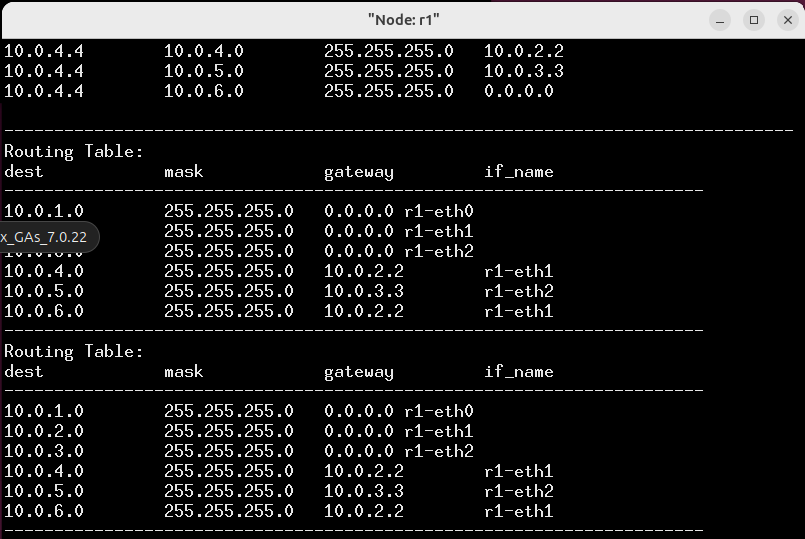
\includegraphics[width=0.8\textwidth]{r1table.png}
    \caption{r1的数据库和路由表}
\end{figure}

\begin{figure}[H]
    \centering
    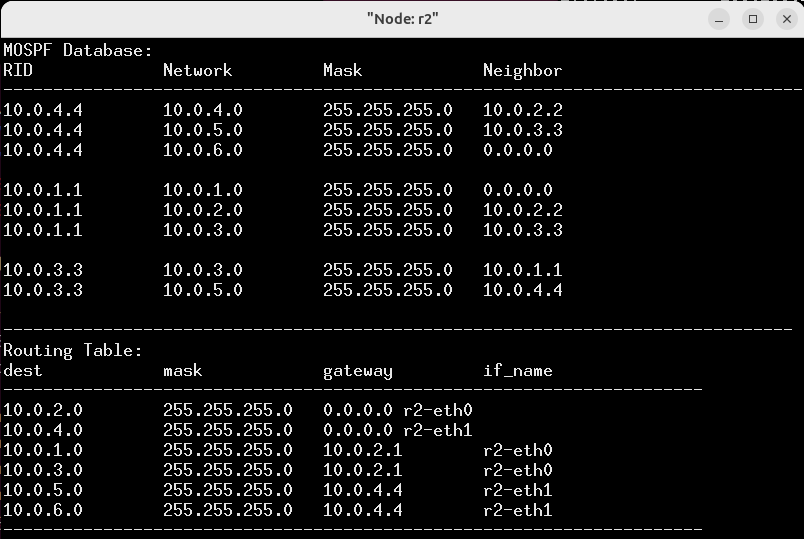
\includegraphics[width=0.8\textwidth]{r2table.png}
    \caption{r2的数据库和路由表}
\end{figure}

\begin{figure}[H]
    \centering
    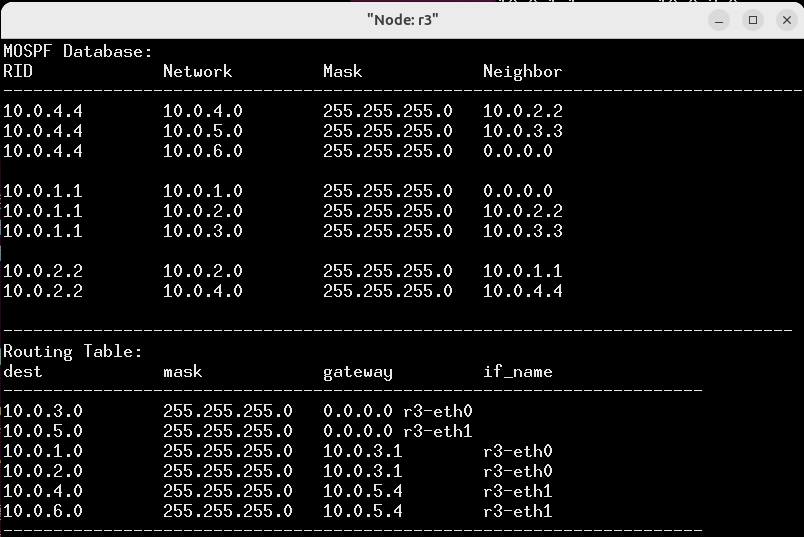
\includegraphics[width=0.8\textwidth]{r3table.png}
    \caption{r3的数据库和路由表}
\end{figure}

\begin{figure}[H]
    \centering
    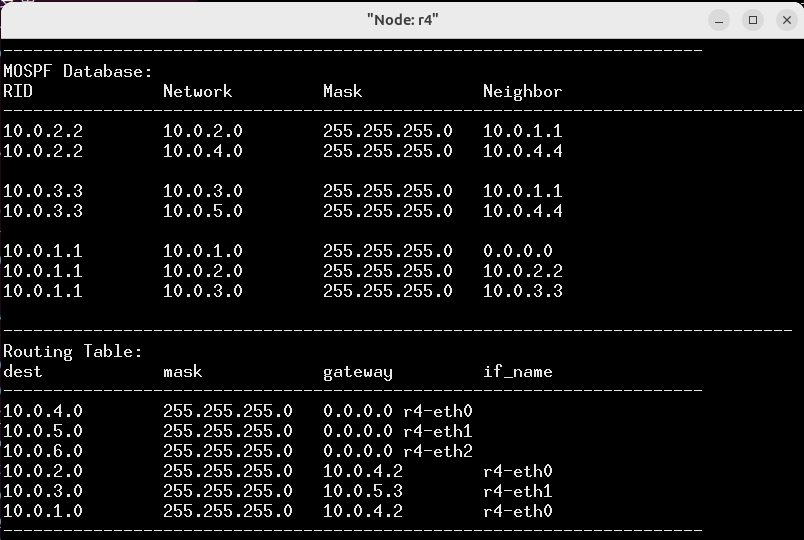
\includegraphics[width=0.8\textwidth]{r4table.png}
    \caption{r4的数据库和路由表}
\end{figure}

可以看出,四个节点的数据库一致,路由表项均存在且正确。

在节点h1上ping节点h2,如下:

\begin{figure}[H]
    \centering
    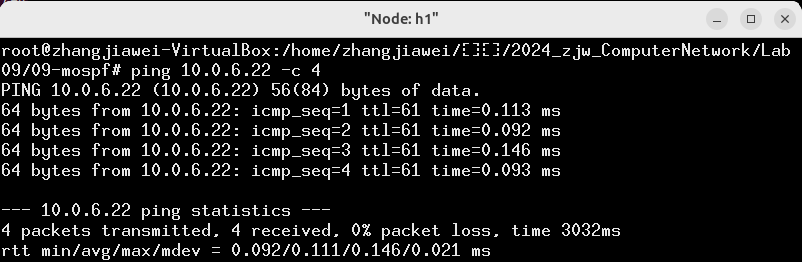
\includegraphics[width=0.8\textwidth]{h1pingh2.png}
    \caption{h1 ping h2}
\end{figure}

在节点h1上traceroute节点h2,如下:

\begin{figure}[H]
    \centering
    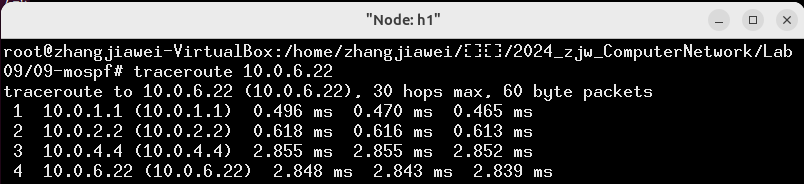
\includegraphics[width=0.8\textwidth]{h1trh2.png}
    \caption{h1 traceroute h2}
\end{figure}

关闭r1和r2之间的链路,等待一段时间后,再次用h1去traceroute节点h2,如下:

\begin{figure}[H]
    \centering
    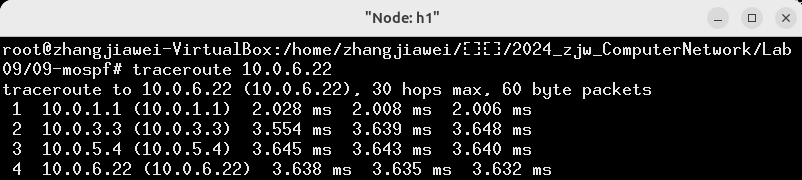
\includegraphics[width=0.8\textwidth]{h1trh2_2.png}
    \caption{h1 traceroute h2 after link down}
\end{figure}

路径发生了变化,说明路由表更新成功,算法正确。

\section{实验总结}

本次实验主要是实现mOSPF协议的Hello/LSU消息的生成和处理,以及路由表的更新计算。实验中需要注意的是,链路状态数据库的一致性,需要在每个节点上都运行mospfd,以便生成一致的数据库;路由表的更新计算,需要使用Dijkstra算法计算最短路径,再根据最短路径更新路由表。实验中还需要注意处理节点失效问题,当链路状态超过40秒未更新时,表明该节点已失效,需要删除对应条目,再更新路由表。我学会了如何实现mOSPF协议的Hello/LSU消息的生成和处理,以及路由表的更新计算,对于理解路由器的工作原理有很大帮助。
\end{document}